\documentclass[11pt]{article}
\usepackage[utf8]{inputenc}
\usepackage{amsmath,amssymb}
\usepackage{tikz}
\usetikzlibrary{arrows.meta, positioning, shapes.geometric, calc}

\begin{document}

\section*{1. Intra-SCC Temporal Feasibility}

Let $u \in C_i$ and $v \in C_i$. Consider a path $P = (u,v)$. We assume that $w$ is the first vertex on the path $P$ that belongs to both the in-tree $T_{\mathrm{in}}^{(i)}$ and the out-tree $T_{\mathrm{out}}^{(i)}$ (note that $w$ could be the center $h_i$).

Consider the transition through $w$ via the edges $(a,w)$ and $(w,b)$:
\begin{align*}
    \lambda(w,b) &= T_i + D_{\mathrm{in}}^{(i)} + d_{\mathrm{out}}(w) \\
    \lambda(a,w) &= T_i + D_{\mathrm{in}}^{(i)} - d_{\mathrm{in}}(a)
\end{align*}

Since $d_{\mathrm{out}}(w) \ge 0$ and $d_{\mathrm{in}}(a) \ge 1$ (assuming unit edge weights and $a \neq w$), it follows that:
\[
    \lambda(w,b) > \lambda(a,w)
\]
This guarantees that the departure time on the out-tree strictly follows the arrival time from the in-tree.

\vspace{1em}
\begin{center}
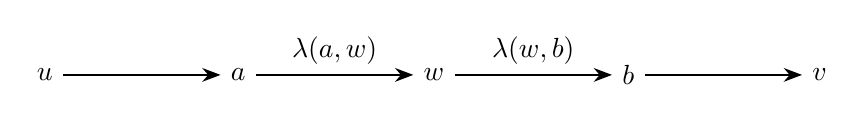
\begin{tikzpicture}[>=Stealth, node distance=2cm, thick]
    \node (u) {$u$};
    \node (a) [right=of u] {$a$};
    \node (w) [right=of a] {$w$};
    \node (b) [right=of w] {$b$};
    \node (v) [right=of b] {$v$};

    \draw[->] (u) -- (a);
    \draw[->] (a) -- node[above] {$\lambda(a,w)$} (w);
    \draw[->] (w) -- node[above] {$\lambda(w,b)$} (b);
    \draw[->] (b) -- (v);
\end{tikzpicture}
\end{center}

\vspace{2em}

\section*{2. Inter-SCC Temporal Feasibility (Cross Edges)}

Let $(a,b)$ be a cross edge where $a \in C_i$ and $b \in C_j$. We analyze the arrival at node $a$ based on its position in $C_i$.

\subsection*{Case 1: If $a \in T_{\mathrm{out}}^{(i)}$}

Consider the path routing through the center $h_i$:
\[
    u \xrightarrow{T_{\mathrm{in}}} h_i \xrightarrow{T_{\mathrm{out}}} x \to a \xrightarrow{\text{cross edge}} b
\]

The departure label for the cross edge is:
\[
    \lambda(a,b) = T_i + D_{\mathrm{in}}^{(i)} + D_{\mathrm{out}}^{(i)}
\]
The departure label from $x$ to $a$ on the out-tree is:
\[
    \lambda(x,a) = T_i + D_{\mathrm{in}}^{(i)} + d_{\mathrm{out}}(x)
\]
Since $d_{\mathrm{out}}(x) + 1 = d_{\mathrm{out}}(a) \le D_{\mathrm{out}}^{(i)}$, we have:
\[
    T_i + D_{\mathrm{in}}^{(i)} + d_{\mathrm{out}}(x) < T_i + D_{\mathrm{in}}^{(i)} + D_{\mathrm{out}}^{(i)}
\]
Thus, the freight arrives at $a$ before the scheduled cross-edge departure.

\vspace{1em}
\begin{center}
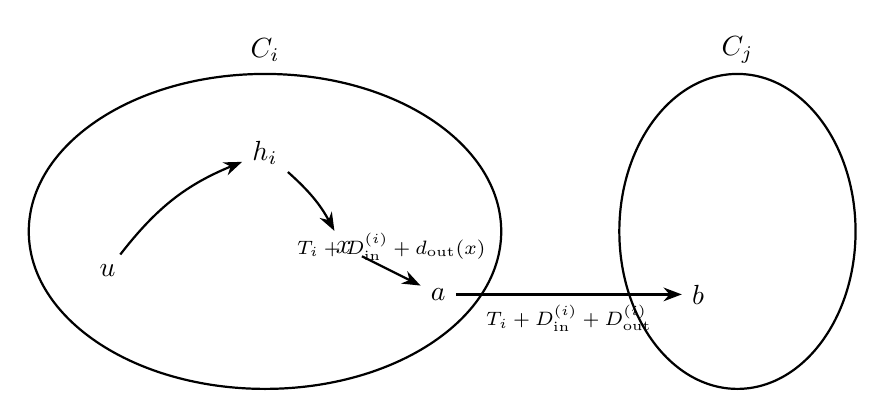
\begin{tikzpicture}[>=Stealth, thick]
    % SCC Ci
    \draw (0,0) ellipse (3cm and 2cm);
    \node at (0, 2.3) {$C_i$};
    
    % SCC Cj
    \draw (6,0) ellipse (1.5cm and 2cm);
    \node at (6, 2.3) {$C_j$};
    
    \node (u) at (-2, -0.5) {$u$};
    \node (hi) at (0, 1) {$h_i$};
    \node (x) at (1, -0.2) {$x$};
    \node (a) at (2.2, -0.8) {$a$};
    \node (b) at (5.5, -0.8) {$b$};
    
    \draw[->] (u) to[bend left=15] (hi);
    \draw[->] (hi) to[bend left=10] (x);
    \draw[->] (x) -- node[above, font=\scriptsize] {$T_i + D_{\mathrm{in}}^{(i)} + d_{\mathrm{out}}(x)$} (a);
    \draw[->] (a) -- node[below, font=\scriptsize] {$T_i + D_{\mathrm{in}}^{(i)} + D_{\mathrm{out}}^{(i)}$} (b);
\end{tikzpicture}
\end{center}

\vspace{2em}

\subsection*{Case 2: If $a \in T_{\mathrm{in}}^{(i)}$}

If node $a$ belongs to the in-tree, its arrival/departure label within $C_i$ relies on $T_i + D_{\mathrm{in}}^{(i)} - d_{\mathrm{in}}(a)$. The cross-edge departure is scheduled at $T_i + D_{\mathrm{in}}^{(i)} + D_{\mathrm{out}}^{(i)}$. Since $-d_{\mathrm{in}}(a) < 0 \le D_{\mathrm{out}}^{(i)}$, the condition holds trivially.

\vspace{1em}
\begin{center}
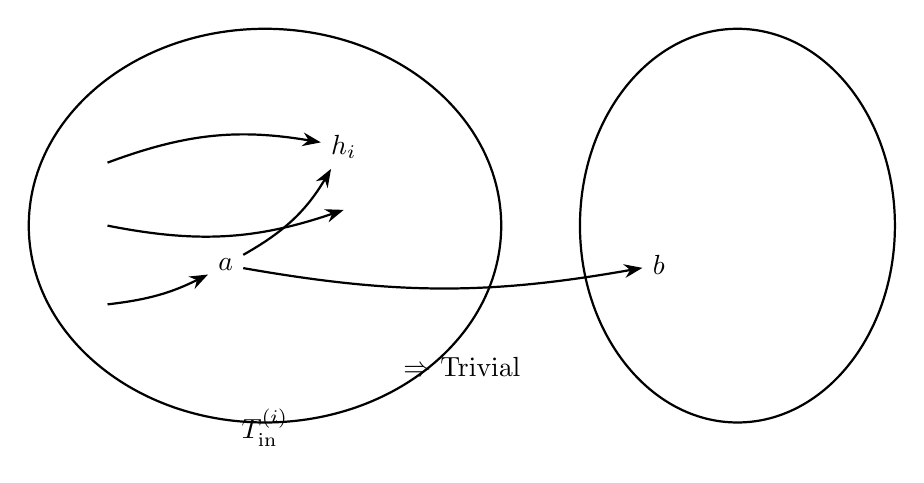
\begin{tikzpicture}[>=Stealth, thick]
    % SCC Ci
    \draw (0,0) ellipse (3cm and 2.5cm) node[below=2.2cm] {$T_{\mathrm{in}}^{(i)}$};
    
    % SCC Cj
    \draw (6,0) ellipse (2cm and 2.5cm);
    
    \node (hi) at (1, 1) {$h_i$};
    \node (a) at (-0.5, -0.5) {$a$};
    \node (b) at (5, -0.5) {$b$};
    
    % In-tree branches
    \draw[->] (-2, 0.8) to[bend left=15] (hi);
    \draw[->] (-2, 0) to[bend right=15] (1, 0.2);
    \draw[->] (-2, -1) to[bend right=10] (a);
    \draw[->] (a) to[bend right=15] (hi);
    
    % Cross edge
    \draw[->] (a) to[bend right=10] (b);
    \node at (2.5, -1.8) {$\Rightarrow$ Trivial};
\end{tikzpicture}
\end{center}

\end{document}
